\documentclass[draft]{homework}

\usepackage{fixme}
\usepackage{graphicx}
\usepackage{hyperref}
\usepackage{minted}
\usepackage{xspace}

\newcommand{\dhcp}{DHCPv6\xspace}
\newcommand{\ip}{IPv6\xspace}
\newcommand{\isp}{ISP\xspace}
\newcommand{\opn}{OPNsense\xspace}


\title{Practical Network Defense - Lab 10}
\subtitle{\ip addressing of ACME co.’s network}
\author{Alessandro Serpi - 1647244}
\date{28 May 2019}


\begin{document}
    \maketitle
    \tableofcontents
    
    
    \pagebreak
    \section{Introduction}
    DHCPv6 prefix delegation is used to assign a network address prefix and automate configuration and provisioning of the public routable addresses for the network.
    
    The router asks the \isp for a network prefix using \dhcp.
    Once assigned, the \isp routes this network to the router, which starts advertising the new addresses to hosts in the network, either via SLAAC or using DHCPv6.
    
    In this environment, only hosts in the DMZ need to receive a global \ip address.
    
    
    \section{Enabling \ip on the firewall}
    In \textit{Interfaces} $\triangleright$ \textit{WAN}, select \textit{\dhcp} in section \textit{\ip Configuration Type}.
    \begin{figure}[H]
        \centering
        
\includegraphics[width=\linewidth]{images/wan-ipv6}
        \label{fig:wan-ipv6}
    \end{figure}
    \vspace{-15pt}
    
    Compile the \dhcp configuration section like in the image.
    Since the \isp\footnote{Since the assignment was carried out in the local environment, the \isp was impersonated by \href{https://klub.com.pl/dhcpv6/}{Dibbler}.} does not spontaneously send Advertise packets, the client must manually ask for the \dhcp server with Solicit messages.
    \begin{figure}[H]
        \centering
        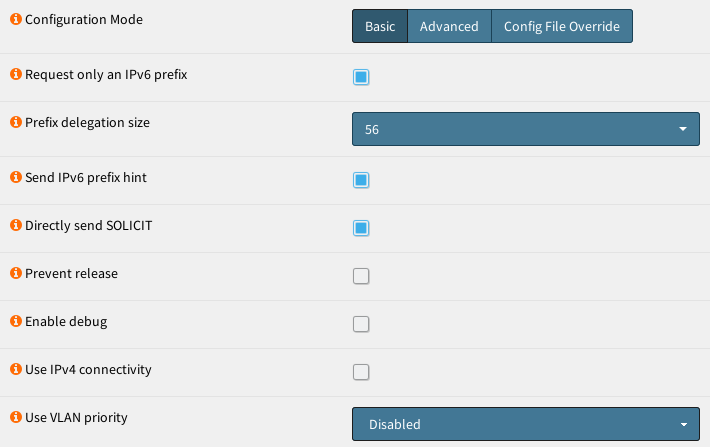
\includegraphics[width=\linewidth]{images/wan-dhcp}
        \label{fig:wan-dhcp}
    \end{figure}
    \vspace{-25pt}
    
    The relevant firewall rules are automatically added by \opn.
    
    
    \section{Enabling \ip on the DMZ}
    The \dhcp server on DMZ interface must be configured with the prefix received on WAN: select \textit{Track Interface} in \textit{Interfaces} $\triangleright$ \textit{DMZ}, section \textit{\ip Configuration Type}.
    \begin{figure}[H]
        \centering
        
\includegraphics[width=\linewidth]{images/dmz-ipv6}
        \label{fig:dmz-ipv6}
    \end{figure}
    \vspace{-15pt}
    
    Leave the just-appeared options (in the bottom of the page) unchanged, only selecting WAN in \textit{\ip interface} if necessary.
    \begin{figure}[H]
        \centering
        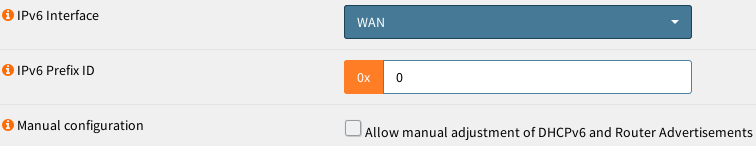
\includegraphics[width=\linewidth]{images/dmz-track}
        \label{fig:dmz-track}
    \end{figure}
    \vspace{-25pt}
    
    The relevant firewall rules are automatically added by \opn.
    
    
    \section{Test of the solution}
    Since the assignment was carried out in a local environment, it made no sense to perform route tracing.
    Instead, since we had complete control over all network components, we started and stopped the \dhcp server and analysed the resulting traffic.
    
    Since the option \textit{Send \ip prefix hint} was checked, the main router did not ask for an arbitrary prefix but for the renewal of a specific one.
    When the server was active, the router received a positive reply (since there were no other clients, the prefix was always available).
    
    Please find attached a successful RENEW/REPLY exchange and the output of \mintinline{sh}{ifconfig em0}, which shows the main router's link-local \ip address.
    
    
    \section{Final remarks}
    \fxnote{TODO}
\end{document}
